\documentclass[a4paper,11pt,onecolumn]{article}



\usepackage{graphicx}

\graphicspath{ {C:/Users/hp/Pictures/} }

\begin{document}

\begin{center}
			\textbf{CHAPTER TWO\\
			LITERATURE REVIEW (WORK IN PROGRESS)\\ Multi-agent-powered model for waste sorting at the public refuse}
		\end{center} 
		\begin{center}
			\textbf{By\\
				Matendo Didas}
		\end{center} 
		
%		CHAPTER TWO}\\\textbf{LITERATURE REVIEW}} \newline \\ By \newline \\ Matendo Didas\\

%\section{Literature Review}
%\label{sec:Literature Review} % (fold)

%\section{Literature }
%\label{sec:Literature Review} % (fold)

%\subsection{Sequential Decion-Making}
%\label{sub:lit-rev_sequential-decion} % (fold)
\textbf{\begin{flushleft}
	2.0 Introduction\end{flushleft}} 
This chapter presents the available literature pertinent to the investigation. It examines the concepts of waste types and production, Artificial Intelligence (AI) in waste management, Sequential Decision-Making (SDM) and its approaches, Multi-Arm Bandit (MAB), Reinforcement Learning (RL), and Monte Carlo Tree Search (MCTS), and their applicability to the research. The Decentralized-Partially Observable Markov Decision Making Processes (Dec-POMDPs) framework is also described in relevance to the current investigation.\\
The analysis of the pertinent linked literature is divided into three themes: 1) AI for Waste Management; 2) Multi-agent system usage; and 3) SDM under Dec-POMDP. Lastly, this chapter concludes with the research gap and contribution, a conceptual overview of the study, and a chapter summary. The purpose of this review of the existing relevant literature was to select the most appropriate agent platforms, algorithms, and multi-agent setup approach, and afterward, to extend choices with the new required functionalities suitable for the context of sorting recyclable waste for our research goals. The essential extension envisioned was the ability to incorporate knowledge to some agents using reasoning models, particularly SDM in multi-agent system environment facets and Dec-POMDPs.\newline\\

\textbf{2.1 Waste Types and Production}\newline
According to Ferronato and Torretta (2019), waste is a significant environmental threat because it can contaminate land, water, and air. According to Chen et al. (2023) and Ukaogo et al. (2020), human activities such as industrial production, construction, agriculture, pollution emissions, consumption, and waste disposal are mostly responsible for its development. Environmental contamination, health hazards, financial losses, and the depletion of waste management resources and expenses can all result from this. Governments, academic institutions, and corporations have adopted waste management techniques like recycling, composting, reusing, employing renewable energy, and embracing green technologies to address these problems (Anuardo et al., 2022). Furthermore, public education and awareness initiatives are thought to be able to lower trash production and motivate people to make more environmentally friendly decisions (Osman et al., 2023).\newline
Different waste classification principles may include grouping waste according to its source, material, or status (Peng et al., 2023). Research on waste sources has shown that the main source of waste is industrial waste (Gaur et al. 2020). Significant environmental pollution results from this waste, which is primarily made up of volatile compounds, waste water, slag, recyclables, and scrap produced during industrial production. These materials contain a variety of hazardous substances, including heavy metals, organic pollutants, and radioactive materials (Patel et al. 2022; Tawfik et al. 2022).\newline
The food sector, wastewater treatment, animal waste, and agriculture all produce organic waste. According to Ren et al. (2018), this kind of trash can be composted, used for value-added projects, or dumped in landfills. Because it contains harmful chemicals like ammonia and chlorine that can pollute the air, water, and soil, organic waste from natural settings can also be dangerous.\newline. The waste states categorize trash into liquid waste (Mekonnen, 2012), organic waste (Sharma et al. 2019), solid garbage (Jha, Dwivedi & Modhera, 2022), hazardous waste (Jha et al. 2022), and recyclable waste (Ren et al. 2018). Recycling, incineration, and landfilling are the treatment methods used for solid waste, which is mostly produced by human activities like mining, manufacturing, and agriculture (Bhatt et al. 2019). The categories of solid waste include hazardous, electronic, medical, construction, domestic, industrial, and agricultural trash (Peng et al. 2023; Vyas et al. 2022). \newline
Toxic, flammable, combustible, radioactive, and corrosive waste, primarily from electronic and biomedical waste, are all considered hazardous waste (Akpan & Olukanni, 2020). Examples of liquid waste include cyanide liquid waste, heavy metal liquid waste, corrosive and alkaline liquid waste, mercury liquid waste, and hexavalent chromium liquid waste. Specifically, 12.4% is made up of corrosive and alkaline liquid waste, 32.2% is made up of organic liquid waste, and 47.9% is made up of heavy metal liquid waste (Ho and Chen 2018). 
The majority of liquid waste is hazardous industrial waste, which can have a serious detrimental impact on the environment and public health if proper control measures are not implemented (Tong & Elimelech, 2016). Trash that can be extracted from the garbage stream and utilized as a raw material to make new goods like paper, glass bottles, and ceramics is known as recyclable waste (Fenta, 2017). Physical retreatment, energy recovery, and biological re-treatment are a few methods of recycling waste (Waheeg, Adesola & Garba, 2022).\newline
Solid trash, hazardous waste, liquid waste, organic garbage, and recyclable waste are the primary categories of waste. Transportation, industry, agriculture, and persons are the primary sources. Recollection, incineration, landfilling, biological, and pyrolysis are some of the treatment techniques. Since recyclable waste is the primary waste type covered by our study that is the only waste kind on which we will concentrate our investigation.\newline \\

\textbf{2.2 Artificial Intelligence in Waste Management}\\

Global trash generation is increasing pollution, waste management, and recycling problems, necessitating innovative approaches to enhance the waste ecosystem, like using artificial intelligence (Fang et al., 2023). By improving the efficiency of garbage collection, processing, and classification, artificial intelligence (AI) has the potential to completely transform waste management. Transportation distance can be cut by up to 36.8 percentage, costs can be reduced by up to 13.35percentage, and time can be saved by up to 28.22 percentage when AI is used in garbage logistics (Fang et al., 2023). Waste may be identified and sorted with an accuracy of 72.8 to 99.95 percentage thanks to AI. Energy conversion, carbon emission assessment, and garbage pyrolysis are all enhanced by artificial intelligence and chemical analysis. Additionally, we describe how artificial intelligence might save costs and boost efficiency in waste management systems for smart cities (Fang et al., 2023).\newline
Intelligent trash cans, image detection, classification robots, predictive models, and wireless detection are examples of AI-based technologies that make it possible to monitor trash cans, anticipate waste collection, and enhance the efficiency of waste processing facilities. Cities can save expenses, increase safety, and lessen the environmental effects of trash management by utilizing AI.\newline 
Research on Human Centered Interfaces (HCI) has just begun to look into garbage sorting and processing technologies and procedures. However, our understanding of how to assist individuals in sorting rubbish in public areas is quite limited. Rather, we observe a design-driven strategy that is largely focused on sustainability through systems and design artifacts that seek to increase users' awareness of their behavior to persuade them to act more sustainably (Lessel et al., 2010). There are three components to our research: (1) prior research on waste management and sorting from different viewpoints and contexts, 2) automatic waste sorting during the execution of Dec-POMDPs, and 3) developing a multi-agent system (smart bin systems, waste-sorting robotic arms, and sensor-based waste monitoring) using AI for SDM techniques.\newline \\
\textbf{Smart Bin Systems:} Traditional trash cans only hold rubbish, and sanitation personnel have to manually check the bins to determine how much trash is inside. For routine trash disposal inspections, this method is ineffective. Furthermore, disease-causing organisms and insects tend to breed on the containers because they are frequently filled (Noiki et al., 2021). Therefore, building smart cities requires the invention of intelligent garbage bin monitoring systems to manage garbage. Two primary features of intelligent garbage cans have been the subject of numerous research studies: automatic waste sorting and monitoring. These studies provide a possible way for cities to have a rubbish-collecting system that works. By using a system on a chip made by Espressif Systems (ESP 8266), intelligent trash can be made that autonomously detects things and establishes thresholds inside the bin. A different node can then receive the collected data for additional processing and analysis (Praveen et al., 2020b).\newline
For instance, Praveen et al. (2020a) created a trash can with two primary pins: an echo pin and a trigger pin that is coupled to the sensor. The top and bottom of the cover are equipped with ultrasonic sensors. Rajathi, Vedhapriyavadhana, and Priya (2019) created a robot trash can that travels in a straight line and has two sensors mounted at the bottom. It features an integrated obstacle sensor on one side that can detect black and trigger a siren to let you know that the trash has been out of storage for a while. Additionally, to determine the trash level, an ultrasonic sensor can be positioned at the edge of the bin (Ogunwolu et al. 2020). The wireless fidelity module will update the web page with the container's state, indicating whether it is full or empty. Using Arduino and wireless fidelity, some researchers create trash cans that divide and track waste (Samann, 2017). It features a metal and non-metal separation that operates automatically. The water level in the bin can be tracked in real-time using NodeMCU and transmitted to the cloud for additional processing and analysis (Saranya et al., 2020).\newline
In conclusion, automatic waste-filling level monitoring and timely user notifications are the primary goals of research on smart garbage cans. Sensors are the main source of the data, which is then sent over the network. Intelligent bin systems can improve the general atmosphere of the city, decrease the spread of diseases, and boost the effectiveness of garbage collection. However, it is difficult to widely market smart garbage cans due to their relatively expensive implementation costs.  To solve this problem, the government might think about providing funds for measures that lower the price of smart trash cans and increase public accessibility. Furthermore, environmental elements like humidity and temperature might have an impact on how often these bins operate. The trash cans must therefore be routinely inspected and maintained by committed staff. As a result, future research must concentrate on creating and promoting smart trash cans, which is also a focus of this study.\newline \\
\textbf{Waste‑Sorting Robotic Arms} For the management of municipal solid waste, garbage classification is highly advised, and the use of robots can significantly increase rubbish classification efficiency. However, to classify rubbish in extremely complex, unexpected, and heterogeneous industrial contexts, robots need sophisticated visual and operational skills (Koskinopoulou et al., 2021). Recent studies have concentrated on increasing the precision and effectiveness of garbage classification robots, which calls for the creation of better cameras and sensors to distinguish between various waste categories as well as enhanced artificial intelligence algorithms for waste classification. One interesting method is to use hyperspectral pictures to find the target region of interest (Xiao et al., 2020). According to earlier studies, robots can handle challenging field situations by incorporating instance segmentation techniques along with simultaneous localization and mapping technologies. They can automatically gather debris from demolition and construction (Wang et al., 2020). \\
Instance segmentation, a type of deep learning (DL) technology, can precisely identify the contours of any object in an image, even rubbish from building and demolition (Chen et al., 2022). Manual collection and classification are frequently ineffective and dangerous due to the complexity of building sites and the massive volumes of garbage produced. As a result, research is being focused on recovering building waste (Yang et al., 2023).\\
Researchers are now exploring ways to incorporate waste-sorting robots into current waste management systems, like using them to separate waste before it is dumped in a landfill. Accordingly, research has proposed a parallel robot model, whose main idea is a gripper that is completely integrated into a robot framework that has four degrees of freedom (Leveziel et al., 2022). To enhance the efficiency of waste-sorting robots, researchers are also investigating the use of optical sensors. For example, a garbage-sorting robot that can precisely recognize and categorize various waste categories has been created with deep learning algorithms and optical sensors (Mao et al., 2022).\\To sum up, robot-based garbage sorting has the potential to greatly improve waste management efficiency, reduce labor costs, and improve the accuracy of refuse classification. In contrast to conventional waste-sorting techniques, some contend that waste-sorting robots are unfeasible because of their high installation and maintenance costs. However, scientists are looking into less costly approaches to building waste-sorting robots, like using less costly materials or building robots that can function in a variety of environments. To make the robot more effective and efficient, efforts are also being undertaken to enhance its sensors, robotic arms, waste sorting algorithms, and structure. In the future, waste-sorting devices will remain very desirable and have a big role in practical applications.\newline \\
\textbf{Sensor‑Based Waste Monitoring:} The method known as sensor-based trash monitoring makes use of sensors to quantify the amount of garbage produced, pinpoint its sources, and assess how well waste management plans are working in a given location. A wireless sensor network is made up of numerous self-organizing wireless sensors that are positioned throughout the system to keep an eye on its environmental or physical characteristics (Gurram, Shariff, & Biradar, 2022).  various sensors, including temperature, humidity, odor, infrared, gas, and sound sensors, are commonly included in wireless sensor network architectures for solid waste treatment systems. Boost the effectiveness of trash management. By using these sensors to track parameters in real-time, the waste treatment process may be effectively managed. To help treat wastewater, for example, sensors can be used to create an electronic nose that measures odor levels in real time (Burgués et al., 2021). \\
Additionally, Sivaprakasam et al. (2020) suggested monitoring nuclear waste glass melts in cold crucible induction melting furnaces in situ using a non-contact microwave sensor. They also created temperature, humidity, and sound sensors to track noise pollution, infrared sensors to gauge the carriages' filling level, and gas sensors to identify dangerous pollutants. Karthikeyan et al. (2017) proposed a Zigbee network-based intelligent waste bin monitoring system where terminal nodes mounted on the trash cans determine the amount of unfilled space. Raaju et al. (2019) proposed that the wireless sensor network be powered by a solar energy collection device to extend the nodes' lifespan.\\
The unavailability of this technology to show the rubbish bin's actual filling levels is its main flaw. To solve this issue, Jino Ramson et al. (2017) proposed a solar-powered wireless monitoring unit equipped with a sensor that detects the can's level when it is empty and sends the data to the unit. The data gathered from several sensor nodes will be sent to the central monitoring station for analysis and visualization to establish a self-powered, direct-connection wireless sensor network solid waste management system (Ramson et al., 2021). In the graphical user interface, a progressive bar is also made to represent the rubbish bin's dynamic unfilled level.\newline \\
\textbf{2.2.1 Manifolds of AI in Waste Sorting} \\
Filtration of waste is necessary to give a recycling method. Waste can be filtered in a variety of methods that appropriately represent the size and cost of the product. Classifying generated garbage and recycled resources is known as source segregation. It is regarded as the ideal material for manually disposing of waste. Over 25 percentage of the positive growth potential can be identified using the trash scattering method. However, more employees are typically needed to process rubbish properly. The optimum use of energy and technology to reduce the risk of respiratory and skin illnesses in humans is this automated method. With a waste disposal rate of only 15 percentage, this is an extremely significant investment.\\
Here, we suggest utilizing the introduction ML algorithm, which has the potential to significantly alter basic methods and achievement levels. To adapt to shifting situations, the machine import algorithm blends preexisting and new conditions and predictors. Its ability to include even the most sensitive and irrelevant sensor data in the decision-making process is one of its greatest benefits. A more advanced system that is stopped by a code that is rarely accessible through the knowledge base may eventually outperform the import system in terms of efficiency.\\
Database assemblers and sensor detectors are PC-powered devices with autonomous operation capabilities. Using a variety of shapes, sizes, colors, levels of contamination, and deterioration, this computer is trained to identify glass, metal, and plastic objects. Every object undergoes a unique sensory nerve sequence. An integrated database is produced by recording the responses related to them. Objectives are used to evaluate each container. The user import algorithms are applied and compared based on the user package parameters. Following the creation of the suggested models, the researcher receives sensor data to assess the precision and consistency. \\
The purpose of the ML algorithm is to learn how to do a task by using pre-set examples and new data. We refer to this as the learning model. Depending on the direct link, it can interpret its reaction from nature. This is known as the principle driven by machine learning. We want to talk about the case studies that the user needs to create a list of potential scenarios when training machine code. Vectors having input and output variables are typically used as examples in the system. Creating a work or pattern that can draw dynamic output extensions is the goal of the learning algorithm. \\
This trash disposal sample's visual attributes include its size, color, sound qualities, and visual acuity. It functions as an alternative to the input model. The material from which the material is obtained and further inputs about the waste collection date can be defined by the container information. It serves as a direct conduit to the output of the system. The garbage cans that send each waste are cut as a result. The integration function is produced by a model-driven learning algorithm once the machine has been fed enough examples. The system chooses the learning strategy and the pertinent parameters. This is crucial for the output's precision, speed, and longevity. AI's many applications in waste sorting include, but are not restricted to:\\
\textbf{A. Image Recognition:} AI systems can analyze waste material photos or videos and distinguish between various waste categories based on visual traits. Large databases of trash picture labels are used to train machine learning models, which enable AI to reliably identify and classify a variety of materials. AI-powered cameras and sensors are used in a waste sorting facility to take pictures of incoming waste moving over a conveyor belt. Real-time picture processing by the AI algorithm allows it to differentiate between metals, glass, paper, and plastics. Each item is subsequently sent to the proper sorting bin or conveyor for additional processing.\\
\textbf{B. Material Identification:} AI-based sensors in a recycling facility identify particular kinds of plastic by scanning mixed garbage. By distinguishing between PET bottles, HDPE containers, and other plastic materials, the AI system maximizes resource recovery and enables tailored recycling procedures. \\
\textbf{C. Adaptive Learning:} ML algorithms are used by AI-powered sorting robots at a garbage sorting facility. The robots are initially trained to sort waste materials that are frequently encountered, but they are constantly learning and adapting to identify and sort new or undiscovered materials that enter the garbage stream, such as composite materials or biodegradable plastics. \\
\textbf{D. Contaminant Detection:} AI-based sensors may identify and eliminate non-paper pollutants like rubber bands, plastic films, and metal clips from a recycling facility that handles paper waste. The AI system ensures greater purity in the finished recycled paper products by identifying and separating the pollutants using machine learning algorithms and image recognition.\\
\textbf{E. Optimization of Sorting Processes:} AI can increase throughput and efficiency in garbage sorting procedures. Artificial intelligence (AI) algorithms can identify the most effective sorting techniques, such as modifying conveyor belt speed, improving sensor settings, or dynamically assigning sorting resources, by evaluating historical data and real-time inputs.\\
\textbf{F. AI in Smart Bins:} a) Fill-Level Monitoring: AI algorithms can monitor the fill levels of waste containers in real-time by analyzing data from sensors placed in smart bins. AI can precisely estimate fill levels and deliver timely notifications for waste collection or maintenance by continuously gathering and analyzing data, b) Dynamic Routing and Optimization: Using real-time fill level data from smart bins, AI can optimize waste collection routes. AI algorithms can dynamically optimize collection routes to reduce trip distance and increase efficiency by evaluating the data and taking into account variables like traffic conditions, proximity, and the fill levels of surrounding bins, c) Predictive Maintenance: By analyzing data from smart bins, AI may anticipate maintenance requirements and take proactive measures to resolve problems. AI algorithms can identify irregularities and forecast when maintenance or repairs might be necessary by tracking a variety of characteristics, including sensor performance, battery life, and connection, d) Contamination Detection: AI can use image recognition techniques or waste composition analysis to find and identify contamination in smart bins. AI algorithms can assist preserve the quality of recyclable materials and lower the danger of contamination by distinguishing between acceptable waste and non-compliant goods, e) Education and Behavior Analysis: AI can examine data from smart bins to learn more about user behavior and waste generation trends. AI algorithms can give waste management authorities useful information to create focused educational programs and promote sustainable waste behaviors by spotting trends and patterns, f) Data Analytics and Insights:  AI may evaluate the information gathered from smart bins to offer insightful information for waste management decision-making. Artificial intelligence (AI) systems can detect patterns, streamline waste management procedures, and assist evidence-based decisions by processing and analyzing vast amounts of data. An overview of AI in trash management is presented in Figure 2.\newline \\
Improve the effectiveness of waste management, lower labor costs, stop the spread of disease, lessen environmental pollution, and perform predictive maintenance on equipment.
Figure 2: Summary of AI in Waste Management\\

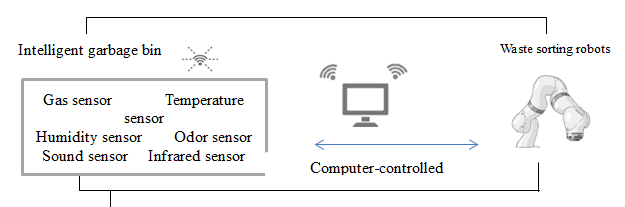
\includegraphics{mab.png}

Figure 2 illustrates how AI is used in trash robotic sorting and the garbage can. \\To avoid bin overflows and optimize waste collection routes, these incorporate real-time garbage bin monitoring. Intelligent rubbish sorting can also lower contamination and increase recycling efficiency. On the other hand, robotic garbage sorting can reduce the requirement for manual labor while enhancing speed and accuracy by using robotic arms to sort waste in recycling plants. To minimize downtime and increase equipment lifespans, AI can also be utilized for predictive maintenance, which predicts when waste-sorting machinery will need maintenance. Finally, to improve the effectiveness of waste collection and processing, artificial intelligence-based waste management optimization can take into account variables like traffic, weather, and population density.\newline \\
\textbf{2.2.2 Artificial Intelligence Models Used in Today’s Era}\\
\textbf{Convolutional Neural Networks (CNNs):} According to Shiri et al. (2023), these deep learning models are a particular class made for handling organized grid-like data, like pictures. CNNs are particularly good at jobs like object detection, medical image analysis, and image and video recognition.  Convolutional, pooling and fully linked layers are among the several layers that make up its architecture (Ahmad et al., 2021). To automatically and adaptively learn spatial hierarchies of features, the convolutional layers apply filters to the input data. This allows them to efficiently capture patterns like edges, textures, and forms. This feature greatly advances the science of computer vision by making CNNs extremely successful for visual recognition tasks. \\
\textbf{Recurrent Neural Networks (RNNs) and Long Short-Term Memory Networks (LSTMs):} RNNs are perfect for jobs like speech recognition and language modeling because they are made for sequence data. Their architecture uses loops to preserve context, but they have trouble with long-term dependencies (Ahmad et al., 2021). With the use of memory cells and gating mechanisms, LSTMs, a kind of RNN, overcome these restrictions and successfully capture long-range dependencies. Because of this, LSTMs are ideal for applications like time-series forecasting and language translation. \\
\textbf{Anomaly Detection (k-means):} K-means clustering anomaly detection finds outliers by measuring their separation from cluster centers. It works well for identifying odd patterns in data and is applied to system monitoring, network security, and fraud detection. Choosing the appropriate number of clusters and managing outliers that may compromise accuracy are difficult tasks (Lu, 2019). The Edge Impulse Studio platform offers tools for preprocessing sensor data, utilizing the k-means algorithm to locate clusters, and identifying anomalies based on departures from the centroids of these clusters (Shiri et al., 2023). This makes it possible for developers to design effective and precise anomaly detection systems that can operate directly on edge devices, which makes it perfect for real-time monitoring and analysis in edge computing and Internet of Things applications.\\
\textbf{Anomaly Detection Gaussian Mixture Models (GMM):} GMM is a statistical technique that models the data distribution as a mixture of Gaussian distributions to discover outliers or anomalies in the data (Ding et al., 2019). To detect anomalies based on low-probability areas of the distribution and capture intricate data patterns, GMM assumes that the data points are produced from several Gaussian distributions. Machine learning models that identify anomalies in sensor data gathered from edge devices can be developed using GMM-based anomaly detection in the context of Edge Impulse Studio (Zong et al., 2018). Tools for preprocessing sensor data, developing GMM models, and deploying them straight onto edge devices are available in Edge Impulse Studio. This makes it possible for developers to produce effective and precise anomaly detection solutions that can operate in real-time on edge devices with limited resources, making them appropriate for a variety of edge computing and Internet of Things applications.\\
\textbf{Reinforcement Learning (RL):} This is the AI model that will be modified for our study. According to Krajna et al. (2022), these models belong to a class of machine-learning algorithms that learn by interacting with an environment through trial and error. In contrast to unsupervised learning, in which the algorithm discovers patterns in unlabeled data, or supervised learning, in which data is labeled, reinforcement learning (RL) learns by getting feedback in the form of rewards or penalties depending on its actions (Krajna et al., 2022; Puiutta & Veith, 2020). To maximize cumulative rewards, the model is guided by this input to gradually enhance its decision-making process. Applications including recommendation systems, automated trading, robotics, and gaming all make extensive use of reinforcement learning (RL), in which agents discover the best course of action by exploring and making use of their surroundings.\\
The challenge of getting an agent to behave in the world in a way that maximizes its rewards can be inferred from the RL model. Instead of being instructed what to do, as is the case with most machine learning methods, a learner (the software) must try many behaviors to see which ones provide the greatest reward.  Actions can influence not only the immediate reward but also the subsequent circumstances and, thus, all subsequent rewards in the most intriguing and difficult scenarios. Consider training a dog a new trick, for instance. We can't tell it what to do, but we may reward or penalize it if it does the appropriate or incorrect action. It must determine what it did to earn the prize or penalty. Similar techniques can be used to teach computers to perform a variety of activities, including scheduling jobs, operating robot limbs, and playing chess or backgammon.\\
According to our research, RL in recyclable garbage sorting will work based on learning via interaction with a multi-agent environment. It is believed that the RL agent, such as a robotic arm or smart bin, will receive feedback based on its activities in the context of our research, which is about sorting recyclable rubbish at public refuse stations. This will enable the agent to gradually improve its methods. The following will be the main elements of the RL system being studied: An agent is a decision-making entity, such as a robotic arm. Environment: The agent's operating environment and the waste sorting system. Actions: The choices the agent may make, such as selecting and classifying a certain kind of garbage. Rewards: Input from the environment that directs the agent's learning process based on its behaviors.\\
According to the conventional RL model, perception and action link an agent to its surroundings. The agent selects an action, a, to produce as output after receiving an indicator of the current state, s, of the environment as input at each stage of interaction. The action modifies the environment's state, and a scalar reinforcement signal, r, tells the agent the value of this state shift. B, the agent, should operate in a way that tends to raise the reinforcement signal's long-term total values. With the help of numerous algorithms that are covered in later portions of this chapter, it can gradually learn to achieve this through methodical trial and error.\newline \\
\textbf{2.4 Sequential Decision Making (SDM)}\\ 
In contrast to prediction, SDM describes how a neural network, referred to as an agent, determines a series of behaviors that can be utilized to engage with an environment and optimize its usefulness (Rizk, Awad & Tunstel, 2018). Sequential decision-making problems are typically modeled as MDPs that satisfy the Markov property (S, A, r, p, γ) (Ou & Bi., 2024). We start establishing the foundation for a formal model of SDM in this section. We describe the agent or decision maker, the environment it interacts with, the behavior it displays, and the potential issues it may encounter. We go on to discuss the methods for dealing with SDM uncertainty. This section also provides a detailed description of the SDM methodologies that are pertinent to the investigation.\\
\textbf{The Agent:} The word "agent" has become overused to the point where it means different things to different groups of people. The system in charge of interacting with the outside environment and making decisions is referred to as an agent in this work. The budget director, the pitcher, and the network monitoring equipment are the agents in the instances from the preceding section. Agents can also be medical devices, software, or robots. A specific economic model, a baseball game, a telephone network, or the floor of an office building is some examples of the environments in which the agents dwell (Kaelbling, 1993). Everything that could change at any time is described by the condition of the environment. The runners' positions, the score, the inning, the current batter's identity, and the number of balls and strikes would all be included in the state in the baseball example. It most likely wouldn't mention the home plate's shape, the number of bases, or the field's color.\\
\textbf{The Environment:}The environment is, in general, everything that is outside of the agent. For this thesis, we assume that environments are unaware of the agent and its objectives rather than being arbitrary or malevolent. More specifically, we assume that the environment is subject to a defined set of rules and changes from one state to another in response to the agent's activities. The transitions may be stochastic, meaning that they don't have to happen every time the agent performs a specific action in a specific state. But over time, the probability governing these stochastic transitions has to stay constant.\\
This notion of environment needs more clarification because it is a little constrictive. The rapidly changing elements of the environment that make up the state and the fixed elements that make up the environment can be distinguished in the majority of real-world issues. Nonetheless, there are frequent elements of the issue that gradually evolve. These can be represented as being static and incorporated into the fixed environment, or they can be treated as part of the state, frequently with a significant increase in the complexity of the state description. \\
A more realistic viewpoint would view the surroundings as non-stationary. Though they are more mathematically complex and contain less formal models, such settings are interesting because they allow for the consideration of a wider range of sequential decision-making problems (Dayan & Sejnowski, 1996). Because of this, prior efforts to deal with non-stationary situations have mostly relied on empirical research (Littman & Ackley, 1991; Sutton, 1991).  Since the theoretical analysis of algorithms is the main focus of this thesis, we limit the discussion to situations that remain constant over time. We do not necessarily assume that the agent has access to a full environmental description, even when we only consider time-invariant settings. In these situations, an agent can frequently find and make use of the time-invariant features; the reinforcement-learning framework models these issues.\\
It is occasionally possible to model external elements that follow their own (not always set) laws as autonomous agents. In the idealized baseball scenario, for instance, the players on the field do their best to obey the coaches' commands; they are a part of the environment. However, because the opposing batter is intentionally unpredictable and confrontational in their decision-making, the environment is best described as having several agents.\\
\textbf{Reward:} Just describing the agent and the environment is insufficient to characterize an SDM problem. The agent must have a reason for acting; in the situations we examine, this reason is to maximize reward. Reward is, in a way, external to the environment and the agent (Zhang et al., 2016).  It serves as a description of the issue that the agent must resolve when interacting with its surroundings. A designer can specify the reward in many sequential decision-making scenarios because they can determine with certainty which states and actions are desirable and which are harmful.  For instance, in the network-analyzer scenario, the agent's rewards might be linked to the money produced and spent by the network's owners; the designer would have incorporated this information into the agent. Since the runs in the baseball example are neither good nor bad in and of themselves, they cannot be regarded as rewards; winning the game is the only thing that truly qualifies. The incentive criterion in the budget example would have to be quite intricate and likely cause a great deal of contention among the management of the company.\\
Although rewards are the foundation of the objective standard by which agents' performance is evaluated, they must be subjectively accessible to agents to have any effect on behavior. One distinguishing feature of the abstract models of environments examined in this thesis is the ability of agents to predict rewards based on their perception of the surroundings. The question of whether incentives can exist in the "undersigned" contexts that biological creatures encounter is an intriguing one.  Specifically, death is the sole real reward signal in a biological system, and the agent detects it too late to be useful. According to simulation experiments, artificial agents can develop their proximal reward functions over many generations, which can be used to predict how good or bad a situation is. In theory, biological agents can also calculate their reward functions (Littman & Ackley, 1991). Additionally, there is proof that certain animal brain regions operate as reward centers and exhibit behavior similar to the reward functions discussed in this thesis. Naturally, it is important to avoid taking these comparisons too literally (Montague & Sejnowski, 1994).\\
\textbf{Policies:} An agent's recommended course of action is called a policy. An agent's policy is generally quite complex, involving behavioral changes that are dependent on long-distance previous occurrences. However, an agent can occasionally act successfully with a much simpler strategy when the environment's structure is known beforehand. One type of policy that is very straightforward is called a plan. In this policy, the agent, with its eyes closed, follows a predetermined course of action, regardless of what it observes. When the agent's initial condition is known beforehand, as is the case, for instance, with manufacturing robots, plans are crucial in totally predictable contexts. A conditional plan allows for some variance in the order of actions chosen. A robot that paints parts, for instance, might be designed to function properly even if it is given a part inverted. Its strategy could look like this: gather the part, check the paint level in the sprayer, ask for additional paint if it's too low, verify the component's orientation, use painting method A if it's right-side up, and use painting procedure B if it's upside down.\\
A stationary policy, commonly referred to as a "universal plan," is an extreme type of conditional plan (Schoppers, 1987). With this kind of policy, there is no set order; rather, the agent looks at the state as a whole at each step and selects the action that is most appropriate given the present state. An agent needs access to a function that returns an action choice for each potential state to carry out such a strategy. Although there are limited theoretical methods to evaluate the effectiveness of a partial strategy, it can be utilized to get around the challenge of creating and modifying complex universal plans (Dean, Kaelbling, Kirman & Nicholson, 1995).\\
Stationary strategies are crucial because of several significant characteristics. First, any partial list of contingencies would be insufficient in highly uncertain contexts because almost any state can follow any other state. Second, it is difficult to envision determining optimal behavior for the intricate success criteria I address in this research without considering action options in every scenario. We frequently use the word "policy" as an acronym for "stationary policy" due to their key significance to algorithms for sequential decision-making. If the agent has to flip a weighted coin to determine what to do, then the policy can also be stochastic. This can be particularly helpful in competitive settings when the agent's degree of unpredictability is crucial.\newline \\
\textbf{2.4.1 Problem Scenarios for Sequential Decision Making} \\
To sort recyclable waste into public trash, we are looking at ways to create policies that maximize a measure of the long-term benefit to an agent in a multi-agent ecosystem. Examples of such agents include robotic arms and smart bins in a particular setting. These policies can be created under two distinct problem situations, planning, and RL, which differ in the knowledge available for policy construction. A comprehensive model of the environment is understood ahead of time in planning. Because of this, the decision-making problem can be divided into two parts: the agent and the planner. The planner is in charge of creating a policy, usually a stationary policy, based on a description of the environment. The agent is then "downloaded" with this policy so that it can be used in the environment. The planner's role is reasonably simple to assess from a typical computer science standpoint because its input and output are specified. This kind of analysis will be carried out during the project.\\
Since the creation of the STRIPS system, one of the main topics in artificial intelligence has been planning (Fike & Nilsson, 1971). The creation of plans for achieving a goal state in a deterministic environment was the main emphasis of early planning research. The use of decision-theoretic planning, which typically involves more intricate environmental models and optimality criteria, has become more popular in recent years. This later work is what sparked our interest in planning.\newline \\
\textbf{2.4.2 Decision-Making Complexity in Real-World Domains}\\
The fields of medicine and the environment are among the crucial areas where poor management choices can have catastrophic social, economic, and environmental repercussions. The intricacy of medical and environmental issues necessitates the creation and use of new instruments that can process not only numerical data but also expert experience and broad public involvement; all of which are essential for decision-making processes (Poch et al., 2004). Real-world system complexity: 
\textbf{The inherent complexity of the systems:} A vast amount of knowledge is involved in these processes, which include intricate relationships between biological, ecological, social, economic, and physical-chemical processes. Moreover, they are stochastic processes that frequently depend on space and time.\\
\textbf{Uncertainty or approximate knowledge:} Numerous qualitative data points are produced by these procedures. With more information or investigation, some of the causes of this uncertainty can be controlled. In other situations, though, ambiguity is unavoidable. The case of self-organizing processes or chaotic behavior serves as an illustration of this. Socio-ecological systems, which have several stakeholders with varying objectives, are similarly characterized by this.  Massive amount of data and information: These fields frequently generate enormous amounts of data and information. Many of the domain's basic facts and principles cannot be accurately described using only deterministic models or mathematical theories.\\
\textbf{Heterogeneity and scale:} Data are frequently heterogeneous because the media in which these processes occur are not uniform and are difficult to describe using quantifiable factors. Furthermore, it is necessary to effectively integrate and manage the various scale times that are inherent to the various process measurements.\\
\textbf{The multiplicity of scales:} Historically, medical and environmental issues have been linked to different timescales and different spatial sizes (local, national, and global). Nonetheless, it is becoming more evident how various scales interact. As a result, it is getting more and harder to promote a single viewpoint that covers all aspects of a system. \newline \\
\textbf{2.4.3 Approaches to Sequential Decision-Making (SDM)}
The MAB strategy is covered in this part along with how it relates to the study topic of developing a multi-agent system for recycling garbage sorting at disposal sites. It contains an overview of MAB, the fundamentals of the MAB methodology, and a thorough explanation of MAB algorithms for making decisions in the face of uncertainty. \\
\textbf{2.4.3.1 Introduction to Multi-Armed Bandits Approach}
The MAB issue, which has its roots in the context of casino gambling machines, seeks to maximize returns by optimizing sequential decision-making (Fu, 2024). Despite its Wild West connotations, the phrase "multi-armed bandit" refers to much more than only shootouts and standoffs (Cai et al., 2023). It features a section where probability, statistics, and state-of-the-art algorithms combine to help people make well-informed decisions and get the most out of their undertakings.  A key idea in optimization and decision-making, the MAB problem encapsulates the exploration-exploitation conundrum seen in numerous real-world scenarios (Ferreira, Schubert & Scotti, 2024). This conundrum entails striking a balance between the necessity to take advantage of established resources for short-term gains and investigating uncharted territory that can provide bigger returns later on (Slivkins, 2019). Since its inception in the early 1900s, the MAB problem has evolved from a theoretical conundrum to a framework that facilitates a broad range of applications in numerous domains, such as recommendation systems, internet advertising, and clinical trials. \\
For algorithms that manage uncertainty while making decisions over time, MAB is a straightforward but incredibly effective paradigm (Slivkins, 2019). In this ML context, an agent must choose actions (or arms) to maximize its total long-term reward (Zhao, 2025). At the start of each round, the agent is provided with some background information about the present situation. It uses this information along with the information acquired from previous rounds to make its judgment. At the end of each round, the agent receives the reward associated with the selected action. An agent is presented with multiple options, or arms, in the MAB problem, each of which gives a reward chosen from an unknown probability distribution. Throughout a series of trials, the agent aims to maximize its cumulative reward (Vermorel & Mohri, 2005). Finding the ideal arm requires finding a balance between using known arms that have produced high rewards in the past and investigating various arms to find out more about their reward distribution.\\
For instance: In the mall, we wish to use RL to assist Baby Robot in finding his way back to his mother. However, he must refuel at a series of power outlets that offer varying degrees of charge before he can begin looking for her. For Baby Robot to swiftly charge and carry on his hunt, we must use strategies from the multi-armed bandit problem to identify the optimal outlet in the shortest amount of time.  There are five power outlets in the charging chamber where Baby Robot has entered. Each of these sockets returns a slightly different amount of charge. If we want the Baby Robot to be charged as quickly as possible, we must find the best socket and use it till the charging process is complete. The only distinction between this and the MAB conundrum is that instead of looking for a slot machine with the biggest payout, we are looking for a power outlet that offers the maximum charge.\newline \\
\textbf{2.4.3.2 MAB Approach Principles}\\
Notably, the MAB is a traditional method for making decisions sequentially in unpredictable situations. Its goal is to determine the best course of action to maximize long-term benefits by means of ongoing testing and observation (Sengupta et al., 2021). Each machine or arm symbolizes a potential choice or course of action, and the payout or probability of winning each arm indicates the probable return of that choice or activity. This simulates the situation of slot machines in casinos.\\
Many people face circumstances similar to the MAB dilemma in real life when choices must be made in the face of uncertainty (Ortega & Braun, 2014). These options could include things like network routing, product recommendations, and ad placement, among other things. A framework for resolving such issues is offered by the Multi-Armed Bandit algorithm, which enables us to make the best choices, given the time and information available. The sentences that follow illustrate some of the fundamental ideas that apply to MAB:\\
o	When an agent chooses an action, we assume that there is at least one action that yields the highest numerical reward and that each action has its reward distribution. As a result, the agent (decision-maker) is unaware of the distinct probability distribution of the rewards associated with each action. Therefore, the agent's objective is to determine which course of action to take to receive the highest reward following a specific sequence of trials.
o	The usual assumption in the MAB issue is that each arm's rewards follow a secret distribution, such as the Bernoulli or Gaussian distributions, among others.
o	Through continuous experimentation and observation, the algorithm seeks to determine the arm that produces the maximum reward to determine the true reward distribution of each arm (Alagumani & Natarajan, 2025).
o	Exploration entails trying out arms that are not yet fully understood in order to learn more about their rewards, whereas exploitation is selecting the arm with the largest reward that is now known in order to maximize immediate earnings. This MAB process necessitates striking a balance between the two'\\
The exploration-exploitation conundrum is at the heart of MAB. More research is required in the early phase of the algorithm to gather sufficient data to estimate the actual rewards of each arm because of the poor understanding of the reward distribution of each arm.\\
The program modifies its estimates in response to the data it gathers over time regarding each arm's rewards. To optimize long-term profits, the algorithm may now turn towards exploitation and select weapons that have performed better. But if exploration is stopped, the algorithm can converge to a locally optimal solution and lose out on better arms. As a result, maintaining the equilibrium between exploration and exploitation within the MAB algorithm is a continuous task. To make the best choices in an unpredictable environment, the algorithm must dynamically modify the exploration-to-exploitation ratio based on available knowledge and historical data.\newline \\
\textbf{2.4.4 MAB Algorithms Comparison for Our Project}\linebreak \\
Various techniques, such as Thompson Sampling, Upper Confidence Bound, and ε-greedy, have been developed by researchers to solve MAB problems. These algorithms have shown differing degrees of good performance in various contexts. The way that MAB algorithms handle the balance between "exploration" and "exploitation" is the main factor that determines how they are categorized and compared. First, some of the most popular MAB algorithms are as follows: \newline \\
\textbf{Epsilon-greedy (E- E-greedy):} In the context of the MAB problem, this is a typical probability-based approach. With this method, exploitation takes place by choosing the currently identified best arm, that is, the one with the highest average reward, with a probability of 1-ε, whereas exploration takes place by randomly selecting an arm with a probability of ε (Zhang et al., 2025). The ε-greedy algorithm specifies an exploration rate ε, which typically falls between 0 and 1. A random integer between 0 and 1 is produced at each stage of the action selection process. A random action is chosen if this number is less than ε; if it is equal to or larger than ε, the best course of action is determined using the body of knowledge. It should be mentioned that this approach increases the possibility of leveraging the gained knowledge by allowing the agent to thoroughly explore unknown states and actions in the early phases of learning and then gradually reducing the exploration rate.\\
The Q-learning (Quality learning) model is one of the many RL models that heavily relies on the ε-greedy algorithm. This method is frequently used in the Q-learning algorithm to choose the subsequent course of action, successfully striking a balance between the agent's learning process and the utilization of learned information. The agent's exploration and exploitation trade-off can be controlled by varying the value of ε, which in turn affects learning speed and final performance.\\
\textbf{The Upper Confidence Bound (UCB):} The fundamental idea behind this value-based method is to give each arm (or option) an upper bound based on past data before selecting the arm with the highest upper bound for exploration or exploitation (Khamaru & Zhang, 2024). The upper bound, represented by the confidence interval, plays a crucial part in the UCB algorithm's reconciliation of the exploration-exploitation trade-off. Maximizing cumulative benefits is its main goal (Ren & Zhang, 2024). Stated differently, the "explore-exploit" approach is used by the UCB algorithm. The algorithm prefers to investigate more arms to gather information in the early stages because of the inadequate understanding of the reward distribution of each arm. The computer gets increasingly precise estimates of the average reward and uncertainty for each arm as data mounts. To maximize the overall reward, the algorithm now leans more toward choosing arms with high average payouts and low uncertainty. The UCB1 algorithm represents the most often used description of the confidence interval in the UCB algorithm. By adding the estimated uncertainty (often a standard deviation or comparable metric) and the average reward for each arm, it determines the UCB.\\
Thompson Sampling (TS): This heuristic algorithm is especially good at resolving the explore-exploit dilemma and is used to handle online decision-making challenges. Its main idea is to use Bayesian probability principles to express uncertainty in the form of probabilities and to probabilistically balance exploration and exploitation when choosing courses of action. Every option or course of action in Thompson Sampling has a corresponding probability model that explains the distribution of potential rewards or returns. The algorithm chooses the course of action with the greater sample return at each decision point by taking a sample from the probability model of each option. This allows the algorithm to select both known-to-perform (exploitation) and possibly high-return (exploration) activities with less up-to-date information (Ma et al., 2024).\newline \\
\textbf{2.4.5 Detailed Analysis of the MAB Algorithms}
The ε-greedy algorithm is a popular exploration-exploitation trade-off technique in reinforcement learning (RL) that permits an agent to make random exploratory decisions with a given probability ε. This method takes advantage of the best technique now in use, which has a probability of 1-ε, and allows for the development of potentially better solutions (Liu, 2024). The following is a thorough examination of the advantages and disadvantages of the ε-greedy strategy:\\
The ε-greedy approach has certain advantages. For instance, it introduces a probability ε to balance exploration and exploitation. Early on in the learning process, the agent can explore to find new and possibly superior tactics. As learning goes on, the agent increasingly cuts back on exploration and bases its decisions on what it has learned. In unpredictable situations, this trade-off enables the agent to swiftly adjust and determine the best course of action.\\ 
Furthermore, the ε-greedy technique doesn't involve complicated parameter tuning or optimization procedures, is easy to implement, and is computationally efficient. This facilitates deployment and implementation in real-world applications. Additionally, the ε-greedy approach works well in a variety of reinforcement learning contexts, including recommendation engines, gaming AI, and advertisement placement. In these situations, the agent must constantly modify its approach in response to feedback from the environment, and the ε-greedy strategy successfully assists the agent in striking a balance between exploration and exploitation.\\
On the other hand, the ε-greedy strategy has a set exploration rate ε, which in some cases might result in either too little or too much exploration. For instance, a constant exploration rate might not adjust to changes in the environment when it gets complicated or unstable, which would prevent the agent from quickly identifying a better course of action. The demands of the agent in various states are not taken into account by the ε-greedy strategy. In certain circumstances, the agent could need to conduct additional research to find new tactics; in other states, the agent might have to base its choices on information that is already known. It is impossible to modify a fixed exploration rate to suit the agent's actual requirements.  In some situations, the agent may miss the global optimal solution and converge to a local optimum since the ε-greedy approach entails a certain likelihood of random exploration in each decision. This issue may be more serious in complex contexts or with limited rewards.\\
Researchers have suggested a few ways to improve the ε-greedy technique to get over its drawbacks. An adaptive exploration rate, for instance, can be used to dynamically modify the ratio of exploration to exploitation in response to changes in the environment and the agent's learning progress; alternatively, the agent's exploration capabilities can be improved by combining different exploration strategies, such as entropy-based exploration and uncertainty-based exploration, among others. Additionally, to fully leverage each algorithm's advantages and enhance overall performance, think about combining the ε-greedy strategy with other reinforcement learning algorithms (such as Q-learning and Policy Gradient, among others). Both MAB and RL issues use the UCB method for exploration. Making judgments based on the average reward and uncertainty (confidence interval) of each action is its central tenet. The benefits and drawbacks of the UCB method are thoroughly examined here (Gao et al., 2023)\\
It has been demonstrated theoretically that the UCB approach converges to the best answer. By adding an uncertainty-related component to the average reward, it determines which actions have the highest upper confidence bound. This strategy strikes a balance between exploitation and exploration, guaranteeing that the agent fully utilizes existing knowledge while simultaneously investigating novel activities. The UCB strategy does not require a fixed exploration rate, unlike the ε-greedy strategy.  Instead, it dynamically modifies the exploration-to-exploitation ratio according to each action's uncertainty and past data. When an action has a high average payoff and low uncertainty, the UCB approach is more likely to exploit it; when an action has a high level of uncertainty, it tends to explore it. The UCB method can better adjust to various activities and surroundings thanks to this adaptable exploration rate. The UCB approach can still be used successfully in contexts with sparse rewards, where the majority of activities result in little to no benefit and just a small number of acts offer substantial value. It can avoid excessive investigation of low-reward actions or local optima by balancing exploration and exploitation by assessing the uncertainty of each action.\\
To calculate the UCB for each action, however, the UCB method necessitates computing the average reward and uncertainty of each action. Sometimes determining the upper confidence bound can be rather difficult and time-consuming, especially when the action space is big or there is a lot of previous data. Due to limitations in processing resources, this could restrict the UCB strategy's practical implementation.  Parameter settings may have an impact on the UCB strategy's performance. For instance, finding a coefficient that strikes a balance between exploration and exploitation is frequently required for determining the upper confidence bound. According to particular jobs and situations, the value of this coefficient must be modified; incorrect settings could result in a decline in performance. Furthermore, the UCB method necessitates the selection of suitable confidence interval widths or levels, which can also affect the strategy's exploration and exploitation behavior. The UCB approach assumes that the distribution of rewards for activities is either constant or varies gradually. The dynamic and non-stationary character of the environment may affect the effectiveness of the UCB method in real-world situations. The UCB method might not be able to adjust in time and identify the best course of action when the environment's reward distribution changes quickly.\\
In practical applications, choosing the right exploration strategy is essential, customized to the particular situation, and combined with other reinforcement learning algorithms and techniques to improve performance. It is important to note that the benefits and drawbacks of the UCB strategy are not absolute and are contingent upon the particular application scenarios and task requirements. The TS method is frequently used to balance exploration and exploitation in multi-armed bandit issues. Its fundamental concept is to select actions based on estimations of the reward distributions for each action, which are maintained through the use of Bayesian inference (Domínguez-Barbero, García-González & Sanz-Bobi, 2023). The following is a thorough evaluation of the benefits and drawbacks of the Thompson Sampling technique\\
Based on past data and approximations of the reward distributions for each action, TS can adaptively modify the ratio of exploration to exploitation. When an action's uncertainty is high, the strategy prefers to investigate it to learn more about it; when the action's average reward is high and its uncertainty is low, the strategy tends to take advantage of it to maximize gains. Because of its versatility, TS can function effectively in a variety of settings and situations. Thompson Sampling can sustain efficient exploration in settings with sparse rewards, where the majority of activities yield little to no reward and only a small number of actions yield substantial gains. It can strike a balance between exploration and exploitation by regularly updating estimates of the reward distributions, preventing over-investigation of low-return behaviors or local optima.\\
There is a strong theoretical basis for TS. The reward distributions for each action are estimated using Bayesian inference, which is a probabilistically plausible method. The strategy's theoretical reliability has also been increased by combining it with other reinforcement learning algorithms to create a number of expanded and enhanced versions.
However, TS might be more computationally demanding than certain straightforward exploration techniques (like ε-greedy). Each action's reward distribution must be estimated and updated, requiring numerous numerical computations and sampling procedures. This processing complexity could become a barrier to its use if the action space is big or there is a lot of historical data.  Parameter settings may have an impact on TS's performance. For instance, particular activities and circumstances require modifications when selecting likelihood functions and prior distributions. Performance may suffer as a result of incorrect parameter adjustments. Determining parameters like the sampling approach and update frequency is another aspect of the strategy that may affect performance. TS may occasionally have a slower rate of convergence. It might need more investigation in the first stage to get enough data because it uses Bayesian inference to update estimations of the reward distributions. Early on, this could lead to less-than-ideal performance, which eventually becomes better.\\
Analyzing an algorithm's advantages and disadvantages in real-world applications is subjective and contingent upon the particular application environment and task specifications. Performance can be enhanced by combining appropriate exploration tactics with various reinforcement learning algorithms and methodologies, which should be selected according to particular situations. Additionally, as research advances, new enhancements and optimization techniques might be able to get around TS's drawbacks and increase its functionality in real-world applications.  A more sophisticated view of these popular MAB algorithms is revealed by further comparison and analysis, which looks at their methodological underpinnings and how they perform in different scenarios. Despite being simple and easy to use by employing a preset probability for exploration, the ε-greedy method frequently fails in non-stationary contexts where flexibility is essential. The simplicity of this algorithm makes it easy to tune, but it may not react well to changes in the reward distribution over time, which could result in less-than-ideal long-term performance.\\
On the other hand, the UCB method performs exceptionally well in situations when precise uncertainty estimations are essential. UCB is especially effective in settings with steady and predictable reward distributions because it efficiently strikes a balance between exploration and exploitation by computing the upper confidence bounds based on statistical confidence. This approach reduces the possibility of missing out on potentially better options because of initial underperformance by making sure that decisions take into account both the degree of uncertainty surrounding each option and historical rewards.\\
Contrarily, TS uses a probabilistic methodology, revising its beliefs about the reward distributions of each choice regularly in response to observed results. In situations when reward probabilities change, this Bayesian approach effectively adapts its selection technique in real-time. Because of its flexibility, TS can continuously improve its choice, which gives it a major edge in dynamic, complicated environments where the reward landscape is always shifting (Thompson, 1933). The efficacy of each algorithm depends on the particular operational needs and environmental dynamics of its deployment. Thus, selecting an algorithm depends on having a thorough awareness of the advantages and disadvantages of each approach in light of the application context, highlighting how crucial it is to match the algorithm's properties with the surrounding circumstances to maximize performance.\\ 
The ε-greedy algorithm will be used for the present project being studied because of its excellent RL support. By allowing agents, such as robots and smart bins, to learn intricate behaviors through trial-and-error, RL can improve garbage sorting by increasing sorting accuracy and lowering contamination in waste bins.\newline \\
\textbf{2.4.6 Other Approaches to Sequential Decision Making}
\textbf{Reinforcement Learning (RL) and Monte Carlo Tree Search (MCTS):} The foundation of RL is a trial-and-error approach where the agent engages with the surroundings. However, MCTS is a strategy that uses random sampling of game states and is based on a heuristic search. The trade-offs between MCTS and RL agents demonstrate the substantial benefit of reinforcement learning; nevertheless, this solution necessitates a lengthy learning period, which is highly dependent on the processing capacity at hand. Although MCTS appears to have fewer requirements, it takes a lot longer to make a judgment. \\
To identify the best choices by sampling a particular model, MCTS was presented as a search and planning framework (Browne et al., 2012; Coulom, 2006). Upper confidence boundaries for trees were one of its earliest iterations. An almost complete revolution in game-playing agents was started by Kocsis & Szepesv ́ari (2006). Significant performance gains over more conventional search techniques could be made, particularly in the game of Go, if an agent has access to an internal mental simulator (Gelly & Wang, 2006; Silver et al., 2016). After demonstrating impressive outcomes, the method was widely adopted in a variety of fields (Browne et al., 2012).\\
Despite being created as a stand-alone algorithm, MCTS's relationship to RL was soon proposed (Silver, 2009). However, the game AI community has not generally adopted this link; therefore it was not immediately evident. The majority of applied researchers were not aware of the linkages between MCTS and RL approaches, and the relationship between the two domains remained relatively hazy. Dedicated game researchers and RL researchers do not share the same vocabulary, which is one of the primary causes of this lack of cross-fertilization. Here, we adopt a much broader perspective and instead address the general difficulties mentioned above, whereas in our earlier work (Vodopivec & Šter, 2014), we just briefly examined the advantages of augmenting MCTS with RL principles. With two primary contributions, we highlight and expand on Silver's (2009) research while attempting to bridge the divide between the MCTS and RL communities.\\
As our initial contribution, we describe the causes of the two communities' distinct development and thoroughly examine the relationship between MCTS and RL. We thoroughly describe the MCTS mechanics with RL theory and analyze which of them are unusual for traditional RL methods and can therefore be understood as novel. By beginning from the MCTS point-of-view, we focus on the AI community and highlight both the similarities and differences between the two fields. Additionally, we review the many MCTS improvements that (intentionally or unintentionally) incorporate RL mechanisms and describe them using RL language. Experts in reinforcement learning may view this initial section of our work as a more thorough background, which may also enable them to recognize some of MCTS's advantages.\\
For agents to learn from experience, reinforcement learning is a well-established paradigm (Sutton & Barto, 1998). An agent acts in an environment while receiving feedback in the form of rewards and observations of the environment's present condition in an RL challenge. The agent's objective is to maximize the anticipated return. To use this information to make better decisions in the future, it attempts to recall or learn which behaviors in which conditions resulted in greater rewards. The MDP formalism is more frequently used in AI research, even though there are several approaches to define the RL problem, such as with operant conditioning in psychology.\\
The RL problem is more challenging than the supervised learning problem since the agent is not instructed on what to do. It must be able to learn from its own experience, that is, samples of interactions with the environment, and it must be able to explore the state space in a trial-and-error manner to find the optimal behavior. Delaying the incentives makes the problem more difficult. The exploration-exploitation dilemma is another significant obstacle, where the agent must choose between exploring lesser-known activities that may prove to be even more advantageous and acting in a way that has historically produced large rewards. This conundrum is at the heart of both bandit and MDP issues.\\
Generally speaking, knowing a value function and then applying it to create an effective policy can address RL problems. Action-value methods are those that work in this manner; the three most popular ones are temporal-difference methods, Monte Carlo methods, and dynamic programming. The latter two fall under the category of sample-based reinforcement learning techniques, which, in contrast to dynamic programming, can learn from sample interactions without the need for an environment model. We concentrate on these in this paper, however, there are other ways to tackle RL problems without explicitly learning the value function, such as using evolutionary algorithms and policy gradient approaches. Wiering and Otterlo provide an overview of numerous cutting-edge RL algorithms (2012).
Furthermore, new research has shown how well RL works for sorting garbage. For example, in order to train RL agents to optimal sorting algorithms based on real-time data, Oliff et al. (2020) simulated a variety of operating scenarios. The use of RL in robotic control was further investigated by Johannink et al. (2019), who demonstrated the technology's promise in both simulated and real-world settings.\\
The application of RL in garbage sorting still faces several obstacles, despite the encouraging outcomes: a) Data Requirements: For RL systems to learn efficiently, they need a lot of data, which might be problematic in some operating environments. b) Integration with Current Systems: It can be difficult to modify RL algorithms so they function flawlessly with the waste management systems of today. c) Scalability: For RL solutions to be widely used, they must be scalable across various facilities and operational sizes. It should be noted that RL offers a substantial chance to improve recycling waste sorting procedures.  RL can result in waste management systems that are more effective and efficient by emphasizing dynamic adaptation, mistake reduction, and real-time decision-making. The use of RL in recycling applications is anticipated to increase as research advances, opening the door for more intelligent waste management strategies, particularly in multi-agent environments like the one suggested in the study.\\
RL has become a game-changing method for trash sorting process optimization, especially in recycling applications. Systems can learn to sort waste materials with the highest accuracy and efficiency by utilizing RL algorithms. This section explores how reinforcement learning can be used practically in recycling, emphasizing how it might improve operational effectiveness.\\
According to our research, smart agents that are outfitted with computer vision systems and deep machine learning algorithms will be able to recognize and categorize various waste types, including plastics, metals, paper, and organic garbage. These agents will include robotic arms, smart bins, and others. Robotic arms are then guided by this information to retrieve the classified objects and place them in the appropriate bins. Through experience and feedback, reinforcement learning enables robots to gradually learn and enhance their sporting abilities. \newline \\
\textbf{2.4.7 Research Influenced by RL and MCTS}\\
Several scholars expanded MCTS to include RL mechanics or the other way around. The researchers' perceptions of the relationship between the two domains vary; some see them as more (or entirely) distinct, others recognize a (strong) connection, and some ignore it and take it for granted.\\
In their RL framework for robots, TEXPLORE, Hester and Stone (2013) use an approach that is comparable to the one we suggested. They only employ UCT to direct the state-space exploration, though and are more interested in their innovative model-learning approach (Hester & Stone, 2010) than in improving MCTS techniques or their relationship to RL. They introduce UCT (λ), which is an extension of the original UCT with λ-returns.  Their approach differs from conventional on-policy MCTS algorithms in that it does not use a play-out phase, does not gradually increase the memory structure (tree), and most importantly does not use the mean of the returns but rather the maximum. Our new algorithm is similar to theirs, but instead of using Q (λ), it uses the Sarsa (λ) algorithm, which memorizes the mean of returns while maintaining all the features of MCTS.\\
A generalization of heuristic search techniques, such as MCTS, is the trial-based heuristic tree-search paradigm put forth by Keller and Helmert (2013). They examine a subset of RL mechanics in their system, namely the substitution of dynamic programming (DP) backups for Monte Carlo backups. With online model learning, their Max UCT method alters the backpropagation to carry out asynchronous value iteration (Sutton & Barto, 1998). \\
Such algorithms are associated with Q-learning (Watkins, 1989) since they rely on the backup of maximum values rather than means, which was initially investigated in an MCTS environment by Coulom (2006) and subsequently by Ramanujan and Selman (2011). They are also connected to the Dyna framework (Sutton, 1990) and adaptive real-time DP (Barto, Bradtke, & Singh, 1995) because of model learning. Following up on the previous work, Feldman and Domshlak (2014) conducted a more thorough analysis of the application of DP updates in MCTS.\\
Khandelwal, Liebman, Niekum, and Stone (2016) developed four UCT variations that use temporal-difference updates in the backpropagation phase concurrently with our study. They evaluate the algorithms using grid-world issues and benchmarks from the International Planning Competition (IPC), and they find that these backup techniques are more advantageous than adjusting the UCT action-selection policy. Their results support ours and offer more justification for using bootstrapping backups in the MCTS environment.\\
One of their algorithms, MCTS (λ), combines UCT and on-policy λ-returns (Sutton & Barto, 1998) to update the estimates in a manner akin to the Sarsa-UCT (λ) method example configuration we employed in our trials. Other than that, Sarsa-UCT (λ) is more general since it keeps all of the RL-based parameters, while MCTS (λ) leaves out the reward discount rate and updates step size. Additionally, the playout phase is not taken into account by MCTS (λ) backups; instead, the algorithm adds all visited states to the search tree. In contrast, Sarsa-UCT (λ) makes a distinction between values that are memorized and those that are not. Finally, the value estimates are normalized using Sarsa-UCT (λ) before being sent to the UCB selection policy.\\
In other research, RL and MCTS are treated more like two distinct algorithmic groups, but their value estimates are combined to create more robust algorithms. Using offline TD-learned values of shape features from the RLGO player (Silver, Sutton, & M ̈uller, 2007) as starting estimates for the MCTS-based player MoGo (Gelly & Wang, 2006), Gelly and Silver (2007) were the first to combine the advantages of both domains. Shortly after, Silver et al. (2007) defined a two-memory architecture known as Dyna-2—an extension of Dyna (Sutton, 1990)—which expanded this "one-time" connection between RL and MCTS to an "interleaving" relationship. \\
As an extension of Dyna-2 for feature learning, Daswani, Sunehag, and Hutter (2014) propose to employ UCT as an oracle to collect training samples that are subsequently used for RL feature learning. To learn a linear function approximator online, Finnsson, H., & Björnsson (2010) utilize gradient-descent TD in Sutton, 1988. They use this to direct the MCTS tree policy and default policy in Cadia Player, a program that has won twice in the General Game Playing competition (Genesereth, Love, & Pell, 2005). \\
General Game Playing competition (Genesereth, Love, & Pell, 2005). 
Using the true online Sarsa (λ) algorithm in (Van Seijen et al., 2016), Ilhan and Etaner-Uyar (2017) additionally teach a linear function approximator online to enhance the performance of vanilla UCT on a series of GVG-AI games. They just utilize it to inform a ε-greedy default policy in the playout. Robles, Rohlfshagen, and Lucas (2011) employ a methodology that is comparable to that of Finnsson and Bj Èornsson (2010). They evaluate the performance of the Othello game after learning the approximator offline, though, and discover that directing the default policy is more beneficial than directing the tree policy.  Osaki et al. (2008) developed the TDMC (λ) method, which enhances TD learning by replacing incentives in nonterminal locations with winning probability. They use traditional Monte Carlo sampling to gather these probabilities, but they recommend the UCT technique for additional research.
Some further scholars recognize a high correlation between RL and MCTS in addition to Veness et al. (2011) and Silver et al. (2012). By expanding the forward search sparse sampling technique (Walsh et al., 2010), an MCTS-like sample-based planner inspired by sparse sampling (Kearns, Mansour, & Ng, 2002), Asmuth and Littman (2011) derive from RL and MDPs while creating the BFS3 algorithm. From a Bayesian standpoint, they reiterate the RL perspective on learning and planning and reaffirm the close relationship between the two. \\
The partially observable Monte-Carlo planning algorithm is created by Silver and Veness (2010) by extending MCTS to partially observable MDPs. Guez, Silver, and Dayan (2013) further improve this algorithm using model-based RL principles to create the Bayes-adaptive Monte-Carlo planner and demonstrate that it performs better than comparable RL algorithms on several benchmarks. By using tile coding, a proven function approximation technique in RL, to improve the UCT play-out phase, Rimmel and Teytaud (2010) create the contextual MCTS algorithm (Sutton & Barto, 1998). Known as "the first extension of MCTS to multi-objective RL," the multi-objective MCTS algorithm was created by Wang and Sebag (2013).
According to Silver et al. (2016), the AlphaGo engine is unquestionably the most effective RL and MCTS estimate combo in contemporary history. It defeated one of the top human Go players in the world in March 2016, overcoming the grand challenge of Go (Gelly et al., 2012). It faced many Go world champions in unofficial online fast-paced bouts at the start of 2017, winning 60 of them and losing none. \\
In a full-length three-game encounter in May 2017, it finally defeated the world's best Go player, winning all three games. However, AlphaGo uses a wide range of AI techniques, such as supervised learning, reinforcement learning, tree search, and—most importantly—deep neural networks (LeCun, Bengio, & Hinton, 2015), which are essential to its success. AlphaGo is considerably more than just a combination of MCTS and RL. Neural networks, both pre-trained offline from a database of matches and self-play, are used to represent their playout policy and value estimators. These networks are then further optimized during online play.  Online search is conducted using a selection method that is similar to UCT and is called the asynchronous policy and value MCTS algorithm. To evaluate locations (and actions), it considers the weighted total of the estimates from Monte Carlo evaluations (playouts) and the pre-trained network.\\
Despite not being directly impacted by MCTS, Veness et al. (2009) demonstrate the advantages of integrating minimax search with bootstrapping backups. Their algorithm, which is a successful example of a study on the intersection of the same two communities that we are also targeting, was able to achieve master-level play in chess, primarily because of the search component.\newline \\
\textbf{2.4.8 Section Summary}
In conclusion, this section has examined a variety of algorithms within the MAB problem, emphasizing notable developments from fundamental techniques like the Greedy and Epsilon-Greedy algorithms to more complex strategies like Bayesian Optimization and Thompson Sampling. These algorithms have substantial theoretical value in the domains of machine learning and reinforcement learning in addition to offering a framework for dealing with practical issues like resource allocation and ad placement. \\
This effort aids in the selection of the best SDM algorithm for the research. According to our comparative research, advanced algorithms give sophisticated answers that are critical in situations with higher decision stakes and complexity, while basic algorithms offer fundamental insights into the exploration-exploitation trade-off. The main conclusions show that Greedy and Epsilon-Greedy algorithms work well in surroundings that are stable and predictable, while they perform poorly in dynamic settings where flexibility is essential. However, because of their probabilistic and confidence-bound methodologies, algorithms like UCB and TS perform very well in situations that call for striking a balance between taking advantages of established resources and investigating novel options. Additionally, when dealing with costly and sparse data, Bayesian Optimization proves to be a potent instrument, offering a strategic framework for well-informed decision-making. The basic ideas of MAB algorithms, including the trade-off between exploration and exploitation, have also been covered in detail in this section.\\
It is important to highlight that the MAB technique is essential for making decisions in difficult situations and has shown great applicability in a variety of industries. Its development from a theoretical idea to practical uses highlights its adaptability and relevance. Sophisticated MAB algorithms are being developed in response to contemporary issues including controlling data uncertainties and adjusting to changing surroundings. A new era of innovation in decision-making mechanisms is being ushered in by the integration of MAB models with more general machine learning and artificial intelligence disciplines, especially in situations that are complicated and constantly evolving (Sawwan & Wu, 2024). MAB algorithms provide useful tools for finding the best choices in unpredictable situations by striking a balance between exploration and exploitation, which propels the growth of related topics.\newline \\
\textbf{2.5 Decentralized-Partially Observable Markov Decision Process (Dec-POMDP) Framework}\\
The Dec-POMDP framework is explained in this section along with how it relates to the present research topic, "Building a multi-agent system for sorting recyclable waste at refuse stations." We give a succinct summary of current advancements that are pertinent to solving the Dec-POMDP problem.\\
Since our topic comprises dispersed multi-agents that must be able to act based on their local information at some time step throughout their learning process in a distant environment setting, it was determined that it was worthwhile to examine Dec-POMDP. The SDM-selected algorithms (RL and MAB) will govern the agents' actions.\\
In a Dec-POMDP, a team of agents works together to maximize a global reward with just local information (Oliehoek, 2012). Because of this, the agents do not experience a Markovian signal while they are acting, meaning that their particular policies are based on their past experiences and are reflected in their behavior (Oliehoek & Amato, 2016). In this section, we discuss current work on decentralized Markov decision processes (Dec-MDPs), in which the control of each agent is influenced by a limited perspective. However, we concentrate on a general framework, expressed as a Dec-POMDP that considers environmental state uncertainty.\\
The scope of decision-making has been expanded in earlier research to encompass numerous agents and to function in scenarios when the state is unknown, like in Partially Observable Markov Decision Processes (POMDPs). Furthermore, rather than studying full RL settings, the majority of research on multi-agent systems under partial observability has concentrated on planning scenarios where the environmental model is already available. By taking into account situations involving numerous agents and state uncertainty, we want to further generalize our research in this study.\\
We pay particular attention to teams of cooperating agents that have a shared objective. 
Such conditions of multi-agents operating in a sparse environment under uncertainty can be defined using the Dec-POMDPs (Pynadath and Tambe, 2002; Bernstein et al, 2002). The study also discusses SDM concerns under Dec-POMDPS and focuses only on planning, with some suggestions for RL methods. The foundation of this model is the idea that, in a two-agent scenario, each agent acts independently at every turn. Depending on what both agents do, the environment's state changes, leading to a reward. A distinct observation of the new state is given to each agent. The consensus is that plans are made offline and subsequently carried out online. Each agent has access to its history of observations and acts throughout the completely decentralized online phase, in addition to its portion of the shared policy created during the planning stage (Chang & Kaelbling, 2003).  The offline planning phase, however, is centralized. Claus and Boutilier (1998) state that we assume that the joint plan is computed by a single computer and then sent to the agents that execute it, online. \newline \\

\textbf{2.5.1 The Relevance of DEC-POMDP Concept}\\

.............Cont's



 






 
 




 


\newline\\

\Cite{slivkins:2024} discusses the \glspl{mab}  problem and its relevance to the research topic. It introduces the concept and discusses various algorithms to achieve decision-making under uncertainty. The term \emph{multi-armed bandit} includes an area where statistics, probability, and cutting-edge algorithms come together to assist in making calculated choices and maximizing their endeavors.
The Multi-Armed Bandit (MAB) problem is a fundamental concept in decision-making and optimization that captures the exploration-exploitation dilemma found in many real-world situations. This dilemma involves balancing the need to exploit known resources for immediate rewards while also exploring unknown options that may yield greater rewards in the future. The MAB problem, which originated in the early 20th century, has transformed from a theoretical puzzle into a framework that supports a wide range of applications across various fields, including online advertising, clinical trials, and recommendation systems. 
The \gls{mab} is a simple yet very powerful framework for algorithms that manage uncertainty while making decisions over time. 

An agent must select actions (or arms) in this machine learning setting in order to maximize its cumulative long-term payoff~\cite{zhao:2025}. The agent is given some context about the current condition at the beginning of each round. It makes its decision based on this data as well as the knowledge gathered from earlier rounds. The reward linked to the chosen action is given to the agent at the conclusion of each round.

In the MAB problem, an agent is given several options (or "arms"), each of which offers a reward selected from an unknown probability distribution. The agent seeks to maximize its cumulative reward across a sequence of trials (Vermorel and Mohri, 2005). In order to choose the best arm, one must strike a balance between exploring different arms to learn more about their reward distribution and taking use of recognized arms that have historically yielded large payouts.

% subsection Sequential Decion-Making (end)

\subsection{Decentralised Partially Observable Markov Decision Processes}
\label{sub:lit-rev_dec-pomdp}

Ref not found
This study outlines the decentralized Partially Observable Markov Decision Process (Dec-POMDP) framework and its relevance to the research topic: "building a multi-agent system for sorting recyclable waste at refuse stations".


A group of agents collaborates to optimize a global reward using only local information in a decentralized partially observable Markov decision process (Dec-POMDP). As a result, the agents do not perceive a Markovian signal during their execution, which means their specific policies are derived from their histories and translated into actions. This paper reviews recent research on decentralized Markov decision processes (MDPs), where each agent's control is influenced by a limited perspective. We focus on a general framework represented as a Dec-POMDP, which accounts for uncertainty regarding the environmental state.


Previous studies have broadened the scope of decision-making to include multiple agents and to operate in situations where the state is unknown, such as in Partially Observable Markov Decision Processes (POMDPs). Additionally, most research on multi-agent systems under partial observability has primarily focused on planning scenarios where the environmental model is already provided, rather than on complete reinforcement learning (RL) settings. In this study, we aim to further generalize this research by considering scenarios with multiple agents and state uncertainty. Specifically, it focuses on groups of cooperative agents that share a common goal. The Dec-POMDPs can be used to define such circumstances (Pynadath and Tambe, 2002; Bernstein et al, 2002).  Additionally, the research addresses issues about sequential decision-making under Dec-POMDPS and concentrates solely on planning, with some recommendations for RL techniques. Lastly, the paper presents the Dec-POMDPS planning model and pertinent Dec-POMDPS scenarios.

This model is based on the principle that, in a scenario involving two agents, each agent acts independently at every stage. The state of the environment changes depending on the actions taken by both agents, resulting in a reward. Each agent receives a unique observation of the new state. There is a common understanding that planning occurs offline, with the plans then executed online. During the fully decentralized online phase, each agent has access to its own history of actions and observations, as well as its share of the joint policy developed during the planning phase (Chang & Kaelbling, 2003). In contrast, the offline planning stage is centralized. According to Claus and Boutilier (1998), we assume that a single computer calculates the joint plan and subsequently distributes it to the agents, who then carry it out online.

We provide a concise overview of recent developments relevant to addressing the Dec-POMDP (Decentralized Partially Observable Markov Decision Process) challenge. In part II, we will explicitly discuss sample scenarios of the Dec-POMDP model. Next, in section III, we will explore Dec-POMDP planning, including actions, states, and observations. Sections IV and V present insights on sequential decision-making within the context of Dec-POMDP and reinforcement learning (RL) respectively. In section VI, we will introduce several notable classes of Dec-POMDPs. Finally, in part VII, we will conclude our discussion.

II. Relevant Scenarios of DEC-POMDP
The Dec- POMDP framework allows modeling important real-world tasks for which the models in the previous researches do not suffice.  The following scenarios depict the cases in which Dec- POMDP can be of great importance:



% section Literature Review (end)
\end{document}